\documentclass[dvipdfmx]{jsarticle}


\usepackage{tcolorbox}
\usepackage{color}
\usepackage{listings, plistings}

%% ノート/latexメモ
%% http://pepper.is.sci.toho-u.ac.jp/pepper/index.php?%A5%CE%A1%BC%A5%C8%2Flatex%A5%E1%A5%E2

%% JavaScriptの設定
%% https://e8l.hatenablog.com/entry/2015/11/29/232800
\lstdefinelanguage{javascript}{
  morekeywords = [1]{ %keywords
    await, break, case, catch, class, const, continue, debugger, default, delete, 
    do, else, enum, export, extends, finally, for, function, function*, if, implements, import, in, 
    instanceof, interface, let, new, package, private, protected, public, return, static, super,
    switch, this, throw, try, typeof, var, void, while, with, yield, yield*
  },
  morekeywords = [2]{ %literal
    false, Infinity, NaN, null, true, undefined
  },
  morekeywords = [3] { %Classes
    Array, ArrayBuffer, Boolean, DataView, Date, Error, EvalError, Float32Array, Float64Array,
    Function, Generator, GeneratorFunction, Int16Array, Int32Array, Int8Array, InternalError,
    JSON, Map, Math, Number, Object, Promise, Proxy, RangeError, ReferenceError, Reflect,
    RegExp, Set, String, Symbol, SyntaxError, TypeError, URIError, Uint16Array, Uint32Array,
    Uint8Array, Uint8ClampedArray, WeakMap, WeakSet
  },
  morecomment = [l]{//},
  morecomment = [s]{/*}{*/},
  morestring = [b]{"},
  morestring = [b]{'},
  alsodigit = {-},
  sensitive = true
}

%% 修正時刻: Tue 2022/03/15 10:04:41


% Java
\lstset{% 
  frame=single,
  backgroundcolor={\color[gray]{.9}},
  stringstyle={\ttfamily \color[rgb]{0,0,1}},
  commentstyle={\itshape \color[cmyk]{1,0,1,0}},
  identifierstyle={\ttfamily}, 
  keywordstyle={\ttfamily \color[cmyk]{0,1,0,0}},
  basicstyle={\ttfamily},
  breaklines=true,
  xleftmargin=0zw,
  xrightmargin=0zw,
  framerule=.2pt,
  columns=[l]{fullflexible},
  numbers=left,
  stepnumber=1,
  numberstyle={\scriptsize},
  numbersep=1em,
  language={Java},
  lineskip=-0.5zw,
  morecomment={[s][{\color[cmyk]{1,0,0,0}}]{/**}{*/}},
  keepspaces=true,         % 空白の連続をそのままで
  showstringspaces=false,  % 空白字をOFF
}
%\usepackage[dvipdfmx]{graphicx}
\usepackage{url}
\usepackage[dvipdfmx]{hyperref}
\usepackage{amsmath, amssymb}
\usepackage{itembkbx}
\usepackage{eclbkbox}	% required for `\breakbox' (yatex added)
\usepackage{enumerate}
\usepackage[default]{cantarell}
\usepackage[T1]{fontenc}
\fboxrule=0.5pt
\parindent=1em
\definecolor{mygrey}{rgb}{0.97, 0.97, 0.97}

\makeatletter
\def\verbatim@font{\normalfont
\let\do\do@noligs
\verbatim@nolig@list}
\makeatother

\begin{document}

%\anaumeと入力すると穴埋め解答欄が作れるようにしてる。\anaumesmallで小さめの穴埋めになる。
\newcounter{mycounter} % カウンターを作る
\setcounter{mycounter}{0} % カウンターを初期化
\newcommand{\anaume}[1][]{\refstepcounter{mycounter}{#1}{\boxed{\phantom{aa}\textnormal{\themycounter}\phantom{aa}}}} %穴埋め問題の空欄作ってる。
\newcommand{\anaumesmall}[1][]{\refstepcounter{mycounter}{#1}{\boxed{\tiny{\phantom{a}\themycounter \phantom{a}}}}}%小さい版作ってる。色々改造できる。

%% 修正時刻: Tue 2022/03/15 10:04:411


\section{2つのテーブルを結合する}

\subsection{内部結合(JOIN句)}

empテーブルの dept\_id は、deptテーブルの id である。

だから、dept\_idをキーにして、二つのテーブルを結合できる。

結合するには \textsf{JOIN}句を使う。

実行例

\begin{tcolorbox}
 MariaDB [sample]$>$ select * from emp \underline{\textsf{join}} dept
 \underline{\textsf{on}} emp.dept\_id = dept.id;
\end{tcolorbox}

これで二つのテーブルが結合される。

\begin{spacing}{0.8}        
\begin{verbatim}
+----+------------+-----+----------+---------+-----+--------+
| id | name       | age | birthday | dept_id | id  | name   |
+----+------------+-----+----------+---------+-----+--------+
|  1 | 菅原文太   |  40 |     1933 | 001     | 001 | 総務部 |
|  2 | 千葉真一   |  34 |     1939 | 002     | 002 | 営業部 |
|  4 | 梶芽衣子   |  26 |     1947 | 002     | 002 | 営業部 |
|  3 | 北大路欣也 |  30 |     1943 | 003     | 003 | 経理部 |
+----+------------+-----+----------+---------+-----+--------+
\end{verbatim}
\end{spacing}

\textsf{join} は \textsf{inner join} と記述できる。
``内部結合''と呼ばれている。

\textsf{on emp.dept\_id = dept.id} は 
emp の dept\_id と dept の id が等しければ、そのレコードを抜き出す。

\rightline{※ emp.dept\_id は empテーブルの dept\_id という意味になる。}

\subsection{表示項目を絞る}

現在は項目を全て表示しているが、これを変更する。

emp表の id, name, age と dept表の name だけを表示させる。


\begin{tcolorbox}
 MariaDB [sample]$>$ select \underline{emp.id, emp,name, age, dept.name}
 from emp join dept \\
 \hspace{6mm} \verb!->! on emp.dept\_id = dept.id;
\end{tcolorbox}

\begin{spacing}{0.8}        
\begin{verbatim}
+----+------------+-----+--------+
| id | name       | age | name   |
+----+------------+-----+--------+
|  1 | 菅原文太   |  40 | 総務部 |
|  2 | 千葉真一   |  34 | 営業部 |
|  4 | 梶芽衣子   |  26 | 営業部 |
|  3 | 北大路欣也 |  30 | 経理部 |
+----+------------+-----+--------+
\end{verbatim}
\end{spacing}        

このように必要な項目のみ表示させることができる。
ただ、name という項目が二つあったり、英語であったりするので、
これを適切な日本語に変える。

それには、\textsf{as句} というのが使える。

たとえば、``emp.name as 名前'' とすると、``emp.neme'' は ``名前'' と表示される。

\begin{tcolorbox}
 MariaDB [sample]$>$ select \underline{emp.id as ID},
 \underline{emp.name as 名前}, \underline{age as 年齢},
 \underline{dept.name as 部署名} \\
 \hspace{6mm} \verb!->! from emp join dept \\
 \hspace{6mm} \verb!->! on emp.dept\_id = dept.id;
\end{tcolorbox}

\begin{spacing}{0.8}        
\begin{verbatim}
+----+------------+------+--------+
| ID | 名前       | 年齢 | 部署名 |
+----+------------+------+--------+
|  1 | 菅原文太   |   40 | 総務部 |
|  2 | 千葉真一   |   34 | 営業部 |
|  4 | 梶芽衣子   |   26 | 営業部 |
|  3 | 北大路欣也 |   30 | 経理部 |
+----+------------+------+--------+
\end{verbatim}
\end{spacing}

さらによく見てみると、この表は部署名の順に並んでいる。
これを ID順に並びかえる。

そのためには \textsf{order句} というのが使える。

たとえば、今回の場合だと、\fbox{\textsf{order by emp.id [asc]}} とすることで、ID順になる。

\textsf{asc} というのは''昇順''という意味で、省略すると asc と指定したことになる。

また、\textsf{desc} と指定すると ''降順'' で並びかえできる。


\begin{tcolorbox}
 MariaDB [sample]$>$ select emp.id as ID, emp.name as 名前, age as 年齢,
 dept.name as 部署名 \\
 \hspace{6mm} \verb!->! from emp join dept \\
 \hspace{6mm} \verb!->! on emp.dept\_id = dept.id \\
 \hspace{6mm} \verb!->! \underline{order by ID};
\end{tcolorbox}

\begin{spacing}{0.8}        
\begin{verbatim}
+----+------------+------+--------+
| ID | 名前       | 年齢 | 部署名 |
+----+------------+------+--------+
|  1 | 菅原文太   |   40 | 総務部 |
|  2 | 千葉真一   |   34 | 営業部 |
|  3 | 北大路欣也 |   30 | 経理部 |
|  4 | 梶芽衣子   |   26 | 営業部 |
+----+------------+------+--------+
\end{verbatim}
\end{spacing}

\textsf{order by emp.id} とするところを \textsf{order by ID} としている。

これは、1行目で \textsf{emp.id as ID} としているので、ID を使うことができるのである。

\newpage
\subsection{外部結合(left outer join / right outer join)}

\subsubsection{左外部結合 left outer join}

この emp表に次のデータを追加する。

\begin{tcolorbox}
 \begin{tabular}{lcl}
  ID & : & 5 \\
  名前 & : & 成田三樹夫 \\
  年齢 & : &  38 \\
  誕生年 & : & 1935 \\
  部署ID & : & (なし) \\
 \end{tabular}
\end{tcolorbox}

\begin{tcolorbox}
 MariaDB [sample]$>$ \textsf{insert into emp (name, age, birthday) values} \\
 \hspace{6mm} \verb!->! \textsf{('成田三樹夫', 38, 1935);}
\end{tcolorbox}

\begin{spacing}{0.8}        
\begin{verbatim}
MariaDB [sample]> select * from emp;
+----+------------+-----+----------+---------+
| id | name       | age | birthday | dept_id |
+----+------------+-----+----------+---------+
|  1 | 菅原文太   |  40 |     1933 | 001     |
|  2 | 千葉真一   |  34 |     1939 | 002     |
|  3 | 北大路欣也 |  30 |     1943 | 003     |
|  4 | 梶芽衣子   |  26 |     1947 | 002     |
|  5 | 成田三樹夫 |  38 |     1935 | NULL    |
+----+------------+-----+----------+---------+    
\end{verbatim}
\end{spacing}


このデータには dept\_id、つまり部署ID がない。たとえば社長とかの場合である。

この状態で 内部結合 をすると、どうなるか?

\begin{verbatim}
MariaDB [sample]> select emp.id as ID, emp.name as 名前, age as 年齢,
    -> dept.name as 部署名 from emp join dept
    -> on emp.dept_id = dept.id
    -> order by ID;
\end{verbatim}

\begin{spacing}{0.8}        
\begin{verbatim}
+----+------------+------+--------+
| ID | 名前       | 年齢 | 部署名 |
+----+------------+------+--------+
|  1 | 菅原文太   |   40 | 総務部 |
|  2 | 千葉真一   |   34 | 営業部 |
|  3 | 北大路欣也 |   30 | 経理部 |
|  4 | 梶芽衣子   |   26 | 営業部 |
+----+------------+------+--------+    
\end{verbatim}
\end{spacing}

結合表には出てこない。

これを図であらわすと、このようになる。

\vspace{3mm}
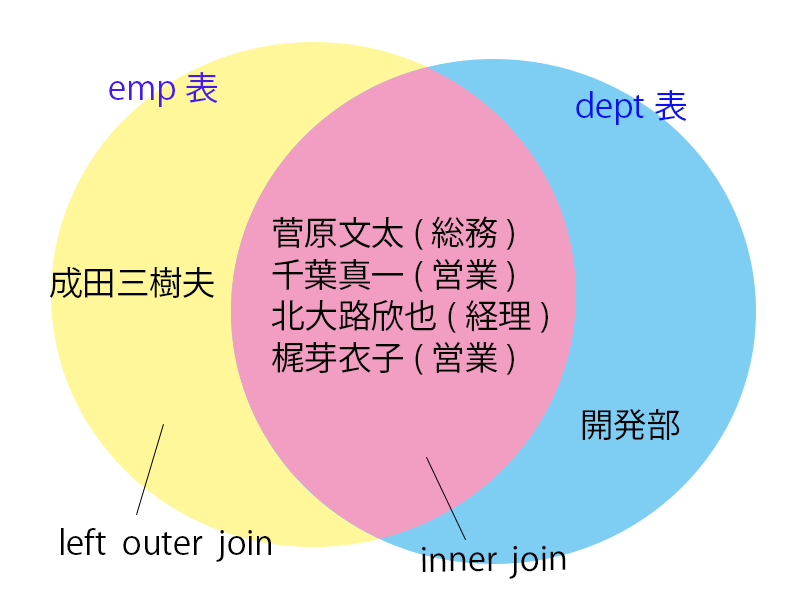
\includegraphics[width=13cm]{../06-mysql/ketsugo.png}
\vspace{3mm}

成田三樹夫は部署IDがないので結合の対象ではない。

こんなときは ''左外部結合(left outer join)'' を使う。

\begin{tcolorbox}
 MariaDB [sample]$>$ select emp.id as ID, emp.name as 名前, age as 年齢, \\
 \hspace{6mm} \verb!->! dept.name as 部署名 from emp \underline{\textsf{left join}} dept \\
 \hspace{6mm} \verb!->! \textsf{on} emp.dept\_id = dept.id \\
 \hspace{6mm} \verb!->! order by ID;
\end{tcolorbox}

\begin{spacing}{0.8}        
\begin{verbatim}
+----+------------+------+--------+
| ID | 名前       | 年齢 | 部署名 |
+----+------------+------+--------+
|  1 | 菅原文太   |   40 | 総務部 |
|  2 | 千葉真一   |   34 | 営業部 |
|  3 | 北大路欣也 |   30 | 経理部 |
|  4 | 梶芽衣子   |   26 | 営業部 |
|  6 | 成田三樹夫 |   38 | NULL   |
+----+------------+------+--------+
\end{verbatim}
\end{spacing}

\subsubsection{右外部結合 right outer join}

また、dept表をみてみると、\textsf{id : '004'} が  \textsf{開発部} であるが、
emp表には dept\_id が '004' である人はいない。

この状態で結合表をつくり、開発部という項目も表示させるには、次のようにする。

\begin{tcolorbox}
 MariaDB [sample]$>$ select emp.id as ID, emp.name as 名前, age as 年齢, \\
 \hspace{6mm} \verb!->! dept.name as 部署名 from emp \underline{\textsf{right join}} dept \\
 \hspace{6mm} \verb!->! \textsf{on} emp.dept\_id = dept.id \\
 \hspace{6mm} \verb!->! order by ID;
\end{tcolorbox}

\begin{spacing}{0.8}        
\begin{verbatim}
+------+------------+------+--------+
| ID   | 名前       | 年齢 | 部署名 |
+------+------------+------+--------+
| NULL | NULL       | NULL | 開発部 |
|    1 | 菅原文太   |   40 | 総務部 |
|    2 | 千葉真一   |   34 | 営業部 |
|    3 | 北大路欣也 |   30 | 経理部 |
|    4 | 梶芽衣子   |   26 | 営業部 |
+------+------------+------+--------+
\end{verbatim}
\end{spacing}



\end{document}

%% 修正時刻: Sat May  2 15:10:04 2020


%% 修正時刻: Wed Aug 11 19:01:36 2021
